% Options for packages loaded elsewhere
\PassOptionsToPackage{unicode}{hyperref}
\PassOptionsToPackage{hyphens}{url}
%
\documentclass[
  man]{apa6}
\usepackage{amsmath,amssymb}
\usepackage{iftex}
\ifPDFTeX
  \usepackage[T1]{fontenc}
  \usepackage[utf8]{inputenc}
  \usepackage{textcomp} % provide euro and other symbols
\else % if luatex or xetex
  \usepackage{unicode-math} % this also loads fontspec
  \defaultfontfeatures{Scale=MatchLowercase}
  \defaultfontfeatures[\rmfamily]{Ligatures=TeX,Scale=1}
\fi
\usepackage{lmodern}
\ifPDFTeX\else
  % xetex/luatex font selection
\fi
% Use upquote if available, for straight quotes in verbatim environments
\IfFileExists{upquote.sty}{\usepackage{upquote}}{}
\IfFileExists{microtype.sty}{% use microtype if available
  \usepackage[]{microtype}
  \UseMicrotypeSet[protrusion]{basicmath} % disable protrusion for tt fonts
}{}
\makeatletter
\@ifundefined{KOMAClassName}{% if non-KOMA class
  \IfFileExists{parskip.sty}{%
    \usepackage{parskip}
  }{% else
    \setlength{\parindent}{0pt}
    \setlength{\parskip}{6pt plus 2pt minus 1pt}}
}{% if KOMA class
  \KOMAoptions{parskip=half}}
\makeatother
\usepackage{xcolor}
\usepackage{longtable,booktabs,array}
\usepackage{calc} % for calculating minipage widths
% Correct order of tables after \paragraph or \subparagraph
\usepackage{etoolbox}
\makeatletter
\patchcmd\longtable{\par}{\if@noskipsec\mbox{}\fi\par}{}{}
\makeatother
% Allow footnotes in longtable head/foot
\IfFileExists{footnotehyper.sty}{\usepackage{footnotehyper}}{\usepackage{footnote}}
\makesavenoteenv{longtable}
\usepackage{graphicx}
\makeatletter
\def\maxwidth{\ifdim\Gin@nat@width>\linewidth\linewidth\else\Gin@nat@width\fi}
\def\maxheight{\ifdim\Gin@nat@height>\textheight\textheight\else\Gin@nat@height\fi}
\makeatother
% Scale images if necessary, so that they will not overflow the page
% margins by default, and it is still possible to overwrite the defaults
% using explicit options in \includegraphics[width, height, ...]{}
\setkeys{Gin}{width=\maxwidth,height=\maxheight,keepaspectratio}
% Set default figure placement to htbp
\makeatletter
\def\fps@figure{htbp}
\makeatother
\setlength{\emergencystretch}{3em} % prevent overfull lines
\providecommand{\tightlist}{%
  \setlength{\itemsep}{0pt}\setlength{\parskip}{0pt}}
\setcounter{secnumdepth}{-\maxdimen} % remove section numbering
% Make \paragraph and \subparagraph free-standing
\ifx\paragraph\undefined\else
  \let\oldparagraph\paragraph
  \renewcommand{\paragraph}[1]{\oldparagraph{#1}\mbox{}}
\fi
\ifx\subparagraph\undefined\else
  \let\oldsubparagraph\subparagraph
  \renewcommand{\subparagraph}[1]{\oldsubparagraph{#1}\mbox{}}
\fi
\newlength{\cslhangindent}
\setlength{\cslhangindent}{1.5em}
\newlength{\csllabelwidth}
\setlength{\csllabelwidth}{3em}
\newlength{\cslentryspacingunit} % times entry-spacing
\setlength{\cslentryspacingunit}{\parskip}
\newenvironment{CSLReferences}[2] % #1 hanging-ident, #2 entry spacing
 {% don't indent paragraphs
  \setlength{\parindent}{0pt}
  % turn on hanging indent if param 1 is 1
  \ifodd #1
  \let\oldpar\par
  \def\par{\hangindent=\cslhangindent\oldpar}
  \fi
  % set entry spacing
  \setlength{\parskip}{#2\cslentryspacingunit}
 }%
 {}
\usepackage{calc}
\newcommand{\CSLBlock}[1]{#1\hfill\break}
\newcommand{\CSLLeftMargin}[1]{\parbox[t]{\csllabelwidth}{#1}}
\newcommand{\CSLRightInline}[1]{\parbox[t]{\linewidth - \csllabelwidth}{#1}\break}
\newcommand{\CSLIndent}[1]{\hspace{\cslhangindent}#1}
\ifLuaTeX
\usepackage[bidi=basic]{babel}
\else
\usepackage[bidi=default]{babel}
\fi
\babelprovide[main,import]{english}
% get rid of language-specific shorthands (see #6817):
\let\LanguageShortHands\languageshorthands
\def\languageshorthands#1{}
% Manuscript styling
\usepackage{upgreek}
\captionsetup{font=singlespacing,justification=justified}

% Table formatting
\usepackage{longtable}
\usepackage{lscape}
% \usepackage[counterclockwise]{rotating}   % Landscape page setup for large tables
\usepackage{multirow}		% Table styling
\usepackage{tabularx}		% Control Column width
\usepackage[flushleft]{threeparttable}	% Allows for three part tables with a specified notes section
\usepackage{threeparttablex}            % Lets threeparttable work with longtable

% Create new environments so endfloat can handle them
% \newenvironment{ltable}
%   {\begin{landscape}\centering\begin{threeparttable}}
%   {\end{threeparttable}\end{landscape}}
\newenvironment{lltable}{\begin{landscape}\centering\begin{ThreePartTable}}{\end{ThreePartTable}\end{landscape}}

% Enables adjusting longtable caption width to table width
% Solution found at http://golatex.de/longtable-mit-caption-so-breit-wie-die-tabelle-t15767.html
\makeatletter
\newcommand\LastLTentrywidth{1em}
\newlength\longtablewidth
\setlength{\longtablewidth}{1in}
\newcommand{\getlongtablewidth}{\begingroup \ifcsname LT@\roman{LT@tables}\endcsname \global\longtablewidth=0pt \renewcommand{\LT@entry}[2]{\global\advance\longtablewidth by ##2\relax\gdef\LastLTentrywidth{##2}}\@nameuse{LT@\roman{LT@tables}} \fi \endgroup}

% \setlength{\parindent}{0.5in}
% \setlength{\parskip}{0pt plus 0pt minus 0pt}

% Overwrite redefinition of paragraph and subparagraph by the default LaTeX template
% See https://github.com/crsh/papaja/issues/292
\makeatletter
\renewcommand{\paragraph}{\@startsection{paragraph}{4}{\parindent}%
  {0\baselineskip \@plus 0.2ex \@minus 0.2ex}%
  {-1em}%
  {\normalfont\normalsize\bfseries\itshape\typesectitle}}

\renewcommand{\subparagraph}[1]{\@startsection{subparagraph}{5}{1em}%
  {0\baselineskip \@plus 0.2ex \@minus 0.2ex}%
  {-\z@\relax}%
  {\normalfont\normalsize\itshape\hspace{\parindent}{#1}\textit{\addperi}}{\relax}}
\makeatother

\makeatletter
\usepackage{etoolbox}
\patchcmd{\maketitle}
  {\section{\normalfont\normalsize\abstractname}}
  {\section*{\normalfont\normalsize\abstractname}}
  {}{\typeout{Failed to patch abstract.}}
\patchcmd{\maketitle}
  {\section{\protect\normalfont{\@title}}}
  {\section*{\protect\normalfont{\@title}}}
  {}{\typeout{Failed to patch title.}}
\makeatother

\usepackage{xpatch}
\makeatletter
\xapptocmd\appendix
  {\xapptocmd\section
    {\addcontentsline{toc}{section}{\appendixname\ifoneappendix\else~\theappendix\fi\\: #1}}
    {}{\InnerPatchFailed}%
  }
{}{\PatchFailed}
\keywords{keywords\newline\indent Word count: X}
\DeclareDelayedFloatFlavor{ThreePartTable}{table}
\DeclareDelayedFloatFlavor{lltable}{table}
\DeclareDelayedFloatFlavor*{longtable}{table}
\makeatletter
\renewcommand{\efloat@iwrite}[1]{\immediate\expandafter\protected@write\csname efloat@post#1\endcsname{}}
\makeatother
\usepackage{csquotes}
\ifLuaTeX
  \usepackage{selnolig}  % disable illegal ligatures
\fi
\IfFileExists{bookmark.sty}{\usepackage{bookmark}}{\usepackage{hyperref}}
\IfFileExists{xurl.sty}{\usepackage{xurl}}{} % add URL line breaks if available
\urlstyle{same}
\hypersetup{
  pdftitle={Employability in Tech: What Gets You A Job Nowadays},
  pdfauthor={Denicia Espinosa Aragon1},
  pdflang={en-EN},
  pdfkeywords={keywords},
  hidelinks,
  pdfcreator={LaTeX via pandoc}}

\title{Employability in Tech: What Gets You A Job Nowadays}
\author{Denicia Espinosa Aragon\textsuperscript{1}}
\date{}


\shorttitle{Employability in Tech}

\authornote{

This paper is a submission the EDLD 654: Machine Learning for Educational Data Science course at the University of Oregon. The data was obtained from Kaggle, an online data science community that host data set for public use. Exact datasource link here: \url{https://www.kaggle.com/datasets/ayushtankha/70k-job-applicants-data-human-resource}

Correspondence concerning this article should be addressed to Denicia Espinosa Aragon. E-mail: \href{mailto:daragon@uoregon.edu}{\nolinkurl{daragon@uoregon.edu}}

}

\affiliation{\vspace{0.5cm}\textsuperscript{1} University of Oregon}

\begin{document}
\maketitle

\hypertarget{research-problem}{%
\subsection{Research Problem}\label{research-problem}}

Jobs in tech are rising in popularity by the day while steadily decreasing in availability at the same rate Picciotto (2023). The news has continuously featured headlines of mass lay-offs at major companies such as Microsoft, Meta, Amazon, General Motor to name a few, totaling over two million tech professional layoffs in 2023 alone Jose (2023). Besides the overwhelming frequency of layoffs, tech jobs are still, again, high in popularity and further continuing to be in high-demand Picciotto (2023). Amongst the change in the job market and massive company reorganizations leading to layoffs, tech professionals must be able to keep up with a changing market, and to do so they need to understand what skills and attributes are needed to stay competitive.

On the other side of the coin, it equally important for companies to know how the industry overall is determining employability, or in other words, what features of a resume contribute the most to getting hired across major tech companies. Understanding employability patterns can address two concerns, reducing the increased labor needed in the hiring process and ensuring equitable decision-making in hiring.

Given the shift in the job market and the surge in job applications, resulting in thousands of submissions for a single job title, companies must streamline operations to enhance efficiency in the hiring process. Efficiency can be provided by extracting crucial information from resumes and assessing it against established criteria used in previous processes for selecting candidates for interviews. Further, extracting demographic data from resumes can help companies evaluate bias in their employment selection processes and make improvements.

The present project intends build and compare multiple machine learning models to effectively predict employment of programmers based on a variety of classic resume components. Additionally, the project will investigate the paramount elements that influence employability.
\#\# Description of Data

The present data was obtained via Kaggle, {``70k+ Job Applicants Data (Human Resource)''} (n.d.) and was created from StackOverlow's annual user-generated survey that includes 73462 software developers in over 180 countries. At download, the variables were standardized to ensure consistency among data points as well cleaned for null responses. Rows in the data represent an individual response from a software developer. Columns represent variables measured for each participant. A few columns were excluded from the dataset due to the lack of detail in what these variables represent or repeated complications in analyses, including, ``Accessibility'', ``HaveWorkedWith'' and ``Employment''. Additionally, in the original data set, the variable ``Country'', representing the origin of each participant, was converted into ``Continent'', representing the continent of origin for each participant. Creating the ``Continent'' variable was conducted reduce dimensionality of the data and improve generalization. Dummy variables were created for all categorical variables and the outcome measure, ``Employed'' was converted into a factor variable. For full description of variables see Table 1.

\begin{table}

\caption{\label{tab:unnamed-chunk-1}Variable Descriptions}
\centering
\begin{tabular}[t]{>{}l>{\raggedright\arraybackslash}p{30em}}
\toprule
Variable & Description\\
\midrule
Age & Participant's age, categorical 
w/ 2 options: lessthan35,greaterthan35\\
Gender & Participant's gender, categorical 
w/ 3 options: Man , Woman, NonBinary\\
Continent & Participant's continent of origin, 
categorical\\
ComputerSkills & Number of computer skills known by 
applicant, integer\\
EdLevel & Education level of the applicant, 
categorical w/ 4 options: Undergraduate, Master, PhD, Other\\
\addlinespace
MainBranch & If the applicant is a professional 
developer, categorical w/ 2 options: Dev, NoDev\\
MentalHealth & Mental Health of the participant, 
categorical w/ 2 options, Yes, No\\
PreviousSalary & Previous salary of the participant, 
integer\\
YearsCode & How long the applicant has been coding, 
integer\\
YearsCodePro & How long the applicant has been coding in
 a professional context, integer\\
\addlinespace
Employed & If the participant was hired or not,  categorical, 
 w/ 2 options: Yes, No\\
\bottomrule
\end{tabular}
\end{table}

\hypertarget{description-of-models}{%
\subsection{Description of Models}\label{description-of-models}}

The outcome variable, Employed, is a binary variable. Therefore, the present project utilizes classification models, specifically using unregularized logistic regression, logistic regression with a ridge penalty, and bagged decision tree for classification. Utilizing this list of models offers a diverse range of linear and non-linear models, each exhibiting distinct levels of variance and bias.
Employing a unregularized logistic regression assumes there is a linear relationship between predictors otherwise known as a less complex model, which ensures a low amount of bias in the model. However, due to the low amount of bias, a unregularized logistic regression model may have higher variance and the trade-off of this balance causes the model to be prone to overfitting.
Deploying a ridge logistic regression adds a penalty to the model coefficients which reduces variance in the coefficients but adds some bias to the model to strike a balance between the variance and bias. Bagged decision trees generally have low bias thanks to the complexity of the model. The hyperparameter for a ridge logistic regression is lambda, which is the penalty placed on the coefficients. For the present dataset, an array of penalty parameters were declared in the attempt to investigate what amount of penalty was optimal.
The last model type, bagging, is short for bootstrap aggregating and describes the process by which multiple models of the same learning algorithm are trained with re-sampling from the same data set. After predictions are created for the multiple models, the predictions are the aggregated to have a final prediction observation for the data set. The hyperparameter for bagged models is the number of bootstrapping samples involved in the model. To evaluate model performance and select optimal model, logloss, area under the ROC (AUG), model accuracy, model precision, and model sensitivity will be compared across the three models. The optimal model will minimize logloss and maximize all other performance parameters.

\hypertarget{model-fit}{%
\subsection{Model Fit}\label{model-fit}}

Based on the model performance measures, the non-regularized logistic regression is the most optimal model to predict employability for software developers, but only by a really small margin. As mentioned previously, the optimal prediction model will minimize logloss, which measures the accuracy of a classification model by penalizing false classifications. The non-regularized logistic regression had a logloss of 0.4437, a few points lower than the ridge logistic regression .4597, and the Bagged Trees logistic regression 0.4597. Further, the non-regularized logistic regression maximized AUC, precision, and true negative rates. AUC also known as area under the ROC curve, measures the model's ability to differentiate between positive and negative classes. Precision is the ratio of correctly predicted positive observations total predicted positive observations. TNR or true negative rates is the measurement how many negatives the model predicts correctly. The non-regularized logistic regression had a AUC of 0.8713, a few points higher than the ridge logistic regression 0.8706, and the Bagged Trees logistic regression 0.8548. For precision scores, non-regularized logistic regression had a score of 0.8001, again few points higher than the ridge logistic regression 0.7995, and the Bagged Trees logistic regression 0.7742. For true negative scores, non-regularized logistic regression had a score of 0.7696, again few points higher than the ridge logistic regression 0.7994, and the Bagged Trees logistic regression 0.7284. Ridge logistic regression performed the best on accuracy (ACC) 0.7847 by a few points compared to non-regularized logistic regression 0.7836 and bagged decision trees 0.7686 while bagged decision trees performed best on true predicted rate (TPR) 0.8032 compared to non-regularized logistic regression 0.7994 and ridge logistic regression 0.7994. (See Table 2 for all numbers) For all analyses, a cut-off point/threshold of .5 was implemented.

\hypertarget{conclusion}{%
\subsection{Conclusion}\label{conclusion}}

While non-regularized logistic regression marginally improved only a few model performance parameters, it consistently outperformed ridge logistic regression and bagged decision trees across the majority of metrics, establishing itself as the optimal model among the three. Bagged decision trees emerged as the least optimal model. In addition to revealing the model performance, it is noteworthy that the most critical parameters vary significantly across each model. For the non-regularized regression, the most important predictor by a landslide was computer skills, again measuring the umber of computer skills known by each participant. Computer skills reported a 100 on the importance scale, possibly indicating over-fitting occurring in this model. Behind computer skills featured previous salary, if a participant was a previously a developer, obtaining a PhD and living in North America to name the first five. For the ridge logistic regression, the most important predictor was obtaining a PhD also will a reported score of 100 on the importance scale. Followed behind a PhD, if a participant was a previously a developer or not, computer skills, and living in South America (See figures 1 and 2).

On a separate note, I learned a ton from this course. My work focuses on how individuals connect with their future self and how we can encourage good decision for a better tomorrow and this course allowed me to think differently about how we investigate open-ended data and predict outcomes in psychology. I hope to use the lessons of this course to create word embeddings and computer a semantic similarity analysis on open-ended descriptions of current and future self and correlate similarity to a measure of future self connection to see if how we describe out current and future self can describe the relationship we feel with our future selves.

\begin{longtable}[]{@{}
  >{\raggedright\arraybackslash}p{(\columnwidth - 12\tabcolsep) * \real{0.4815}}
  >{\raggedright\arraybackslash}p{(\columnwidth - 12\tabcolsep) * \real{0.0864}}
  >{\raggedright\arraybackslash}p{(\columnwidth - 12\tabcolsep) * \real{0.0864}}
  >{\raggedright\arraybackslash}p{(\columnwidth - 12\tabcolsep) * \real{0.0864}}
  >{\raggedright\arraybackslash}p{(\columnwidth - 12\tabcolsep) * \real{0.0864}}
  >{\raggedright\arraybackslash}p{(\columnwidth - 12\tabcolsep) * \real{0.0864}}
  >{\raggedright\arraybackslash}p{(\columnwidth - 12\tabcolsep) * \real{0.0864}}@{}}
\caption{\label{tab:unnamed-chunk-3}Model Performance for All Models}\tabularnewline
\toprule\noalign{}
\begin{minipage}[b]{\linewidth}\raggedright
Model
\end{minipage} & \begin{minipage}[b]{\linewidth}\raggedright
LL
\end{minipage} & \begin{minipage}[b]{\linewidth}\raggedright
AUC
\end{minipage} & \begin{minipage}[b]{\linewidth}\raggedright
ACC
\end{minipage} & \begin{minipage}[b]{\linewidth}\raggedright
TPR
\end{minipage} & \begin{minipage}[b]{\linewidth}\raggedright
TNR
\end{minipage} & \begin{minipage}[b]{\linewidth}\raggedright
PRE
\end{minipage} \\
\midrule\noalign{}
\endfirsthead
\toprule\noalign{}
\begin{minipage}[b]{\linewidth}\raggedright
Model
\end{minipage} & \begin{minipage}[b]{\linewidth}\raggedright
LL
\end{minipage} & \begin{minipage}[b]{\linewidth}\raggedright
AUC
\end{minipage} & \begin{minipage}[b]{\linewidth}\raggedright
ACC
\end{minipage} & \begin{minipage}[b]{\linewidth}\raggedright
TPR
\end{minipage} & \begin{minipage}[b]{\linewidth}\raggedright
TNR
\end{minipage} & \begin{minipage}[b]{\linewidth}\raggedright
PRE
\end{minipage} \\
\midrule\noalign{}
\endhead
\bottomrule\noalign{}
\endlastfoot
Non-Regularized Logistic Regression & 0.4437 & 0.8713 & 0.7836 & 0.7957 & 0.7696 & 0.8001 \\
Logistic Regression with Ridge Penalty & 0.4597 & 0.8706 & 0.7847 & 0.7994 & 0.7677 & 0.7995 \\
Logistic Regression with Bagged Trees & 0.4597 & 0.8548 & 0.7686 & 0.8032 & 0.7284 & 0.7742 \\
\end{longtable}

\begin{figure}
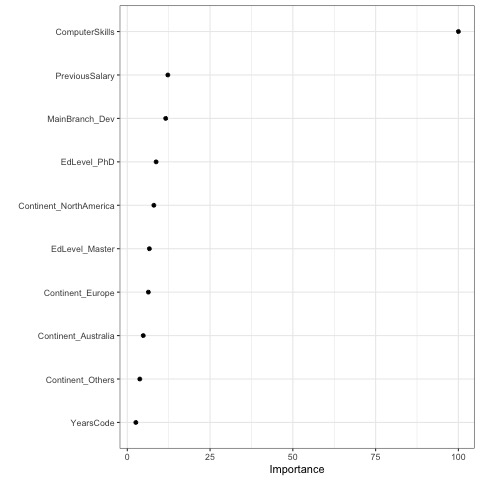
\includegraphics[width=1.6in]{edld_final_project_dfea_files/figure-latex/unnamed-chunk-4-1} \caption{ }\label{fig:unnamed-chunk-4-3}
\end{figure}
\begin{figure}
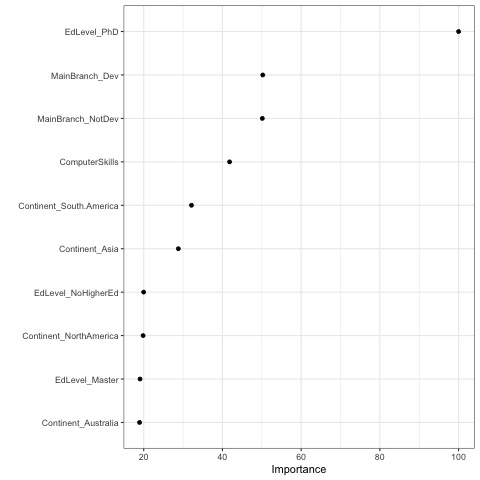
\includegraphics[width=1.6in]{edld_final_project_dfea_files/figure-latex/unnamed-chunk-4-2} \caption{ }\label{fig:unnamed-chunk-4-4}
\end{figure}

\newpage

\hypertarget{references}{%
\section{References}\label{references}}

\hypertarget{refs}{}
\begin{CSLReferences}{1}{0}
\leavevmode\vadjust pre{\hypertarget{ref-noauthor_70k_nodate}{}}%
70k+ job applicants data (human resource). (n.d.). Retrieved December 6, 2023, from \url{https://www.kaggle.com/datasets/ayushtankha/70k-job-applicants-data-human-resource}

\leavevmode\vadjust pre{\hypertarget{ref-jose_tech_2023}{}}%
Jose, B. (2023, December 7). Tech layoffs 2023: Job cuts deepen as spotify, amazon, yahoo and others lay off staff {\textbar} technology news - the indian express. Retrieved December 7, 2023, from \url{https://indianexpress.com/article/technology/tech-news-technology/tech-layoffs-spotify-amazon-layoffs-9056846/}

\leavevmode\vadjust pre{\hypertarget{ref-picciotto_tech_2023}{}}%
Picciotto, R. (2023, July 7). Tech roles are still `the most in-demand,' says job market expert---but you need these skills to land them. {CNBC}. Retrieved December 6, 2023, from \url{https://www.cnbc.com/2023/07/07/tech-jobs-are-still-the-most-in-demand-says-employment-market-expert.html}

\end{CSLReferences}


\end{document}
